\section{Software empleado en el proyecto}
\subsection{ROS}
ROS (Robotic Operating System) consite en un framework para la robótica sobre el que desarrolladores de cualquier 
ambito pueden aportar soluciones modulares a los sistemas de forma general. La modularidad de ROS hace que desarrollar 
un nuevo sistema o prototipo pueda ser una tarea tan sencilla como interconectar módulos de otros desarrolladores con 
los propios.\\
Esta característica lo hace idoneo para un proyecto como este en el que el uso de técnicas de percepción, 
mapeado, localization, etc, complejas se escapa del alcance; y solo sea necesario el desarrollo de modulos específicos de este robot
que sean capaces de comunicarse con aquellos más complejos y sean capaces de proporcionarle los datos necesarios para implementar los
algoritmos de SLAM.
\subsubsection{Computación distribuida con ROS-Multimaster Package}
Las técnicas de SLAM a testear en el robot desarrollado son computacionalmente costosas. De manera genérica a los metodos de SLAM visual usados, 
para cada frame capturado por la camara el algoritmo extrae `features' de la imagen, las alamacena y compara los conjuntos con los de otro frame. 
Entre ambos frames el algoritmo calcula una matriz de transformación homogenea con la cual se es capaz de saber, al menos localmente, cuanto y como se ha
desplazado el robot. Sumado a eso cada algoritmo tiene su forma propia de localizar globalmente en el mapa creado al robot. Todo este coste computacional es
imposible asumirlo desde una Raspberry-Pi, por lo que surge la necesidad de hacer el procesado en un servidor remoto al robot en tiempo real con las 
dificultades que eso conlleva, entre ellas y la mas importante, la sincronización de datos.\\
Bajo estas condiciones de diseño y restricciones aparece una solución de la comunidad: ROS multimaster\_fkie. La premisa que lo rige es simple, dado un sistema mutirobot
cada elemento mantiene la ejecución de 2 nodos locales, \textit{master\_discovery} y \textit{master\_sync}; el primero es el encargado de mantener una lista del resto 
de \textit{roscores} disponibles en la red y de publicar el suyo propio como activo. El otro es el encargado de suscribir su \textit{core} los nodos de otros \textit{cores}.\\
Des esta forma todos tienen acceso de una forma hasta cierto punto `real-time' a los recursos del resto. 
\begin{figure}[!ht]
    \centering
    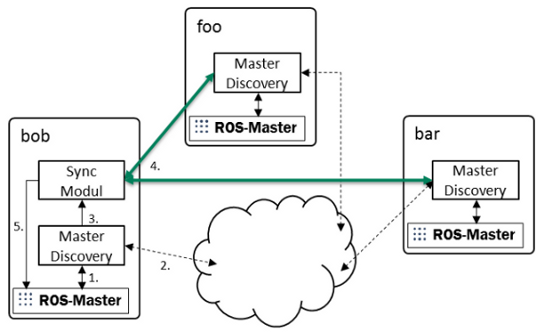
\includegraphics[width=0.6\textwidth]{images/ros_multimaster.png}
    \caption{Esquema del funncionamiento básico del paquete Multimaster}
\end{figure}\\
En este proyecto su integración se ha llevado a cabo lanzando en la Raspberry-Pi y en otro PC los nodos correspondientes siendo la Raspberry-Pi la 
suministradora de información y el PC el encargado de procesarla.
\subsubsection{Interfaz con IMU}
Qué hace, como se procesan los datos y que se publica.
\subsubsection{Interfaz con encoders}
Mismito que lo de la IMU
\subsubsection{Odometría}
Explicar qué se hace, qué y donde se publica y a quién se suscribe
\subsubsection{Interfaz Raspberry-Pi/Arduino}
Qué hace, a quién se suscribe y donde publica el qué
\subsubsection{Interfaz Arduino/Motores}
Same old same old
\subsection{Implementación filtro estadístico}
Introducción de porqué es interesante y eso, lo de vender la moto as usual
\subsubsection{Filtro de Kalman Extendido}
Background teorico que coma espacio, poner la imagen del filtro esa con colores bonicos y eso
\subsubsection{ROS-Robot Localization Package}
pues eso, lo mismo de lo otro, como funca y tal
\subsection{Arquitectura general del sistema}
Aqui lo de rqt\_plot and eso
